%%%%%%%%%%%%%%%%%%%%%%%%%%%%%%%%%%%%%%%%%%%%%%%%%%%%%%%%%%%%%%%%%%%%%%%%%%%%%%%%
%2345678901234567890123456789012345678901234567890123456789012345678901234567890
%        1         2         3         4         5         6         7         8

\documentclass[letterpaper, 10 pt, conference]{ieeeconf}  % Comment this line out if you need a4paper
%\documentclass[a4paper, 10pt, conference]{ieeeconf}      % Use this line for a4 paper

\IEEEoverridecommandlockouts                              % This command is only needed if 
                                                          % you want to use the \thanks command

\overrideIEEEmargins                                      % Needed to meet printer requirements.

% See the \addtolength command later in the file to balance the column lengths
% on the last page of the document

% The following packages can be found on http:\\www.ctan.org
\usepackage{graphics} % for pdf, bitmapped graphics files
\usepackage{epsfig} % for postscript graphics files
\usepackage{mathptmx} % assumes new font selection scheme installed
\usepackage{times} % assumes new font selection scheme installed
\usepackage{amsmath} % assumes amsmath package installed
\usepackage{amssymb}  % assumes amsmath package installed
% \usepackage{comment}
% \usepackage{algorithm,algpseudocode}
% \usepackage{resizegather}
% \usepackage{flexisym}
\usepackage{dblfloatfix}    % To enable figures at the bottom of pag
\usepackage{subcaption}
\usepackage{mathtools}
% \usepackage[square,numbers]{natbib}

% TODO: french letter in name
% \usepackage{inputenc} 

\title{\Large \bf Social RL: Socially Compliant Navigation in Crowds
with Reinforcement Learning}

\author{% <-this % stops a space
\thanks{This work was supported by [?]}% <-this % stops a space
% \thanks{$^{1}$L is with, 
% {\tt\small b.d.researcher@ieee.org}}%
% \thanks{$^{*}$Equal contribution}       
\thanks{Visual Intelligence for Transportation Laboratory, Ecole Polytechnique Federale de Lausanne (EPFL)
, CH-1015 Lausanne,
        {\tt\small \{ \}@epfl.ch}}%
}

\begin{document}

\bstctlcite{IEEEexample:BSTcontrol}

\maketitle
\thispagestyle{empty}
\pagestyle{empty}

\pdfminorversion=4  
%%%%%%%%%%%%%%%%%%%%%%%%%%%%%%%%%%%%%%%%%%%%%%%%%%%%%%%%%%%%%%%%%%%%%%%%%%%%%%%%
\begin{abstract}
This electronic document is a template. The various components of your paper [title, text, heads, etc.] are already defined on the style sheet, as illustrated by the portions given in this document.

\vspace{5cm}

\end{abstract}


%%%%%%%%%%%%%%%%%%%%%%%%%%%%%%%%%%%%%%%%%%%%%%%%%%%%%%%%%%%%%%%%%%%%%%%%%%%%%%%%
\section{INTRODUCTION} \label{sec:intro}

With the rapid growth of machine intelligence, robots are envisioned to expand habitats from isolated environments to social spaces that are shared with humans and other embodied agents. Traditional approaches for robot navigation often view the moving agents nearby as a static obstacle \cite{fox_dynamic_1997} or react to them through a one-step lookahead \cite{berg_reciprocal_2008}, resulting in short-sighted and unnatural behaviors. In order to navigate through a crowd in a socially compliant manner, robots need the ability to understand the behaviors of the others while making its movement decision. 

Navigation with social etiquettes is, however, a very challenging task. As communications among agents (e.g. robots, pedestrians, bikers) are not widely available, robots need to perceive and anticipate the evolution of the crowd that can involve complex interactions. Research works in trajectory prediction have proposed several hand-crafted or data-driven methods to model the agent-agent interactions \cite{helbing_social_1995,alahi_social_2016,vemula_social_2017,gupta_social_2018}. In a addition to the predictive model, how to integrate the interaction knowledge into the decision-making process poses another challenge as well. 

\begin{figure} [t]
  \captionsetup{font=small}
  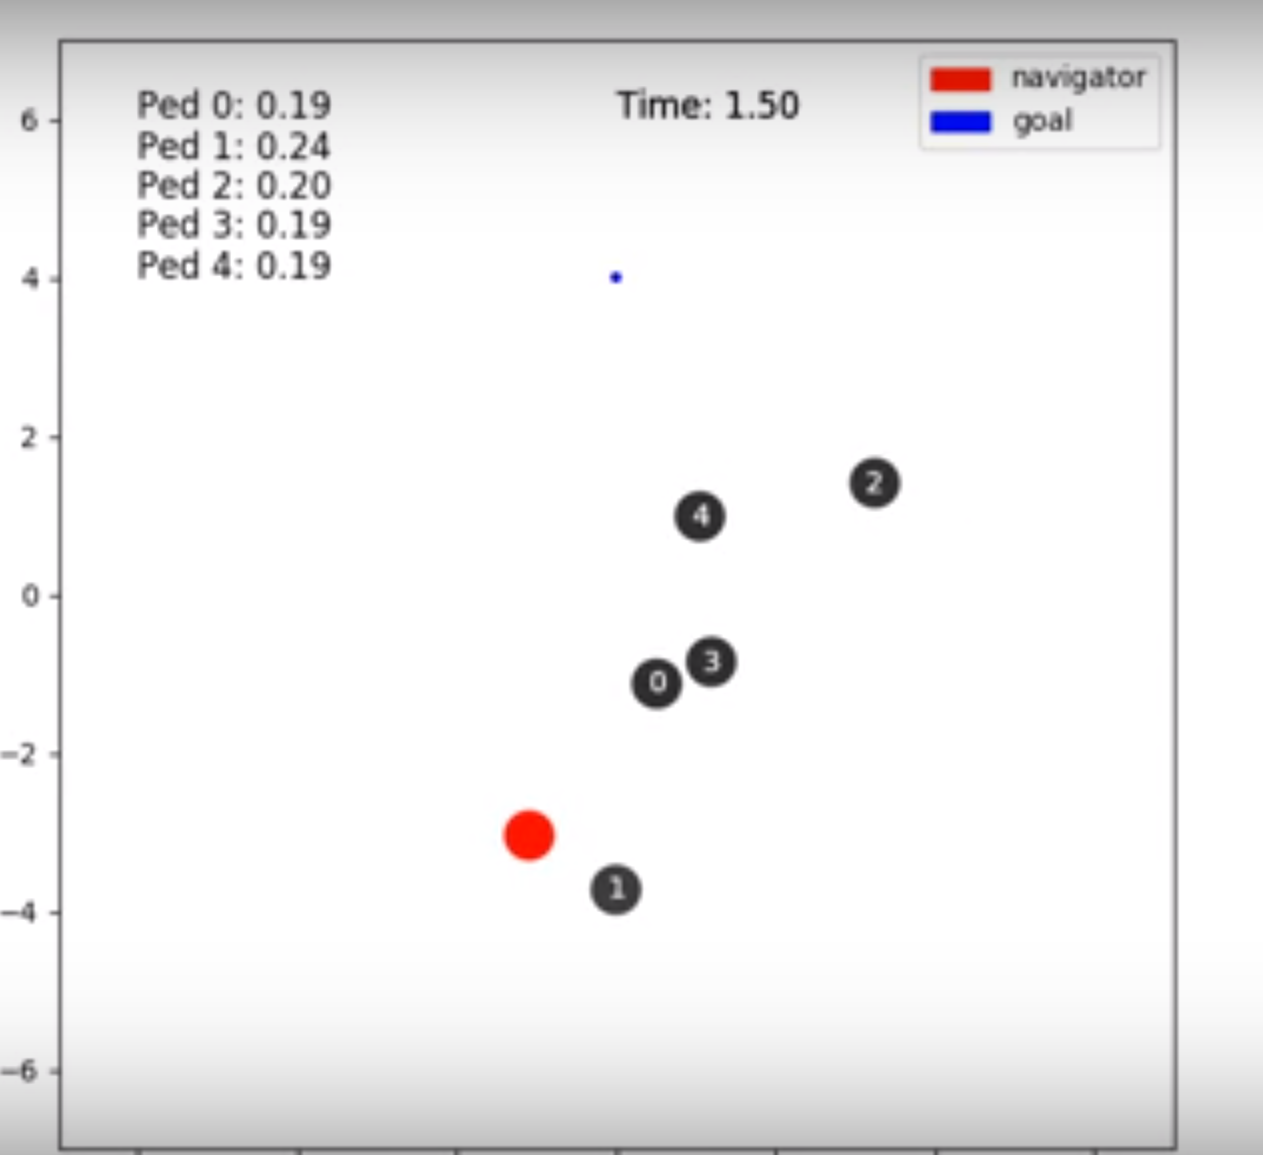
\includegraphics[width=0.2\textwidth]{figures/overview}
  \caption{TODO: Illustration of the socially compliant navigation in a crowded scene.}
  \label{fig:overview}
\end{figure}

Earlier works split the prediction and planning into two separate steps, attempting to identify a safe trajectory distant from the forecasted regions of the other agents for a few steps \cite{bennewitz_learning_2005,aoude_probabilistically_2013}. However, these untraversable regions can be very large in a crowded scene and cause the freezing robot problem \cite{trautman_unfreezing_2010}. To cope with it, jointly obstacle avoidance methods that plan the paths of all the interactive decision-makers simultaneously are proposed, in hope to make the navigation rooms cooperatively \cite{trautman_unfreezing_2010}. Though conceptually desirable, these methods suffer from the computational costs as well as the behavior stochasticity of the neighbors in practice. 

As an alternative, the reinforcement learning method has been used to train a policy that implicitly encodes the interactions and cooperations among agents. While great progress has been made in recent works \cite{chen_decentralized_2016,chen_socially_2017,long_towards_2017,everett_motion_2018}, existing models are limited in two aspects. i) The joint impact of the nearby agents on the navigator is usually aggregated by a simplified model on top of the pariwise interactions, such as maximum operator or LSTM. ii) They are focused on the one-way interactions from the crowd to the navigator but omit interactions within the crowd that can shape the hidden state of each neighboring agent and eventually affect the navigator. These limitations may degrade the capacity of the cooperative planning-based reasoning in complex and crowded scenes. 

In this work, we propose a novel pooling module for the reinforcement learning method, aiming to learn a socially compliant navigation policy in complex scenes. Inspired by \cite{alahi_social_2016,gupta_social_2018,vemula_social_2017}, we first extract the features of the pairwise social interaction between the navigator and each neighbor and subsequently use the soft attention to learn the importance of these interactions. In addition, we encode the impact of intra-interaction on each agent by a local occupancy map. Based on a social state concatenating these interactions, a navigator is trained to navigate through a crowd and learn a value network, which is used to evaluate the scenarios consisting of various group interactions and provide a cooperative navigation policy. An extensive set of experiments shows that our approach can effectively learn to perceive the behaviors of the other agents and navigate through them in a socially compliant manner, outperforming the state-of-the-art methods. 

\section{BACKGROUND} \label{sec:background} 

\subsection{Related Work}

Existing works on cooperative navigation have been extensively focused on the joint obstacle avoidance. Reactive policies such as RVO \cite{berg_reciprocal_2008} and ORCA \cite{van_den_berg_reciprocal_2011} seek the joint collision-free velocities under the reciprocal assumption, which have been successfully applied to the distributed multi-agent systems. \cite{trautman_unfreezing_2010} propose a noval Interacting Gaussian Process (IGP), which models the trajectory of each individual as a Gaussian Process and introduces an interaction potential to couple the individual GP for collaboration. The polices built upon hand-crafted cooperation models, however, sometimes fail to obey the human-like patterns in crowded scenarios.

Another line of works uses the imitation learning approach to program a socially compliant policy from demonstrations. \cite{tai_socially_2017} and \cite{long_deep-learned_2017} developed policies that map raw depth images and lidar measurements to actions respectively by directly mimicing the demonstrations. Instead of behaviorior cloning, maximum entropy learning inverse reinforcement learning method was used to learn the features of the observed human behaviors \cite{roy_feature-based_2013, kretzschmar_socially_2016, pfeiffer_predicting_2016}. The learned model of these methods highly depend on the quality of demonstrations, which can be very resources consuming. 

Reinforcement leanring for navigation in dynamic enviroment. 
- Raw sensor input
- Agent-level state
Our we extend social interaction model for the agent-level state 

\vspace{2cm}

Social representation is intensively studied by the deep learning approach in recent years. 
- LSTM
- Graph 
- Soft attention 
Our work extend the social pooling from sl prediction to rl planning

\vspace{2cm}

\subsection{Problem Formulation}

Consider a navigation task that a robot moves to a goal destination through a crowd of pedestrians $\{1,2,\dots,n\}$. It can be formulated as a decision making problem through a sequence of observations, action, and reward triplets\cite{chen_decentralized_2016,chen_socially_2017,everett_motion_2018}. Let $\bold{s}_t $, $\tilde{\bold{s}}_t = [\tilde{\bold{s}}_t^1, \tilde{\bold{s}}_t^2, \dots, \tilde{\bold{s}}_t^n]$ denote the state of the robot and the pedestrians at time $t$ respectively. Specifically, the full state of the robot is defined as $ \bold{s} = [\bold{p}, \bold{v}, r, \theta, \bold{p_g}, v_{pref}]$ and the observable state of a pedestrian is defined as $ \tilde{\bold{s}}_i = [\bold{p}, \bold{v}, r]$, where $\bold{p}=[p_x,p_y]$ and $\bold{v}=[v_x,v_y]$ are the vectors of location and velocity in the $2D$ plane, $r$ is the radius. We assume that the robot is aware of its unobservable state including the heading angle $\theta$, goal position $\bold{p_g}$ and preferred speed $v_{pref}$ and that the robot velocity can be achieved by the action command $\bold{a}_t$ immediately, $\bold{v}_t = \bold{a}_t$. The joint state for the robot navigation at time $t$ is defined as $\bold{s}_t^{jn} = [\bold{s}_t, \tilde{\bold{s}}_t]$. 

The desired navigation policy, $\pi : \bold{s}_t^{jn} \mapsto \bold{a}_t$, is to maximize the objective function without violating the constraints:
\begin{subequations} \label{eq:optimization}
\begin{align}
& \underset{\pi(\bold{s}^{jn})}{\text{argmax}}
& & \mathbb{E}[\sum_{t=0}^T R_t | \bold{s}_0^{jn}, \bold{p}_g, \pi] \label{eq:obj} \\
& \text{subject to} 
& & \bold{p}_T = \bold{p}_g \label{eq:goal} \\
&&& \bold{p}_{t+\Delta t} = \bold{p}_{t} + \Delta t \pi(\bold{s}_{t}^{jn}) \label{eq:kinematics} ~ & t = 0, \Delta t, \dots, T \\
&&& \left\Vert \bold{p}_t - \tilde{\bold{p}}_t^i \right\Vert >= r + \tilde{r}^i & i = 1, 2, \dots, n \label{eq:safety}
\end{align}
\end{subequations}
where (\ref{eq:obj}) is the expected total reward that the robot can obtain in the navigation task, (\ref{eq:goal}) is the goal constraint, (\ref{eq:kinematics}) is the kinematics of the robot, (\ref{eq:safety}) is the safety constraint, $T$ is the time when reaching the goal, and $\Delta t$ is the time step interval. 

The reward function is defined to penalize the collision and uncomfortable distances and award the task accomplishment, 
\begin{equation}
    R_t(\bold{s}_t^{jn},\bold{a}_t)= 
\begin{dcases}
    -??? & \text{if} ~~ d_t < 0 \\
    -0.? + d_t? & \text{else if} ~~ d_t < 0.2 \\
    1 & \text{else if} ~~ \bold{p}_t=\bold{p}_g \\
    0 & \text{otherwise} 
\end{dcases}
\end{equation}
where $d_t$ is the minimum seperation distance between the robot and the pedestrians during the time period $[t-\Delta t,t]$. 

The problem (\ref{eq:optimization}) can be tackled by a reinforcement learning method that seeks a optimal policy 
\begin{equation} \label{eq:RL}
\begin{split}
\pi^{*}(\bold{s}_t^{jn}) = & \underset{\bold{a}_t}{\text{argmax}} ~ R(\bold{s}_t^{jn},\bold{a}_t) + \\
& \gamma^{\Delta t \cdot v_{pref}} \int_{\bold{s}_{t+\Delta t}^{jn}} P(\bold{s}_t^{jn},\bold{a_t},\bold{s}_{t+\Delta t}^{jn}) V^*(\bold{s}_{t+\Delta t}^{jn}) d\bold{s}_{t+\Delta t}^{jn}
\end{split}
\end{equation}
where $\gamma \in [0,1)$ is a discount factor, $P(\bold{s}_t^{jn},\bold{a_t},\bold{s}_{t+\Delta t}^{jn}) $ is the transition probability from time $t$ to time $t+\Delta t$, during which the robot takes the action $\bold{a_t}$. The state transition probability can be viewed as a trajectory prediction model for a short period of time. 

\begin{figure} [t]
  \captionsetup{font=small}
  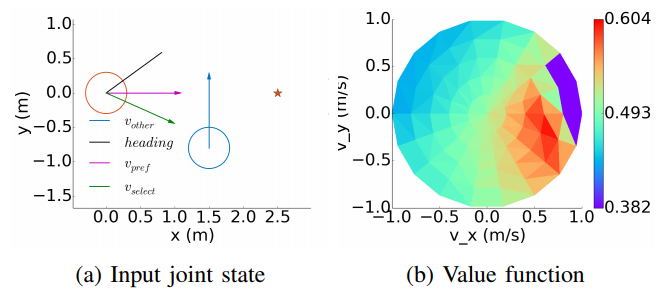
\includegraphics[width=0.5\textwidth]{figures/vf} 
  \caption{TODO: Value function estimation for a navigation task in a dense crowd.}
  \label{fig:overview}
\end{figure}

The optimal value function $V^*$ is an estimate of the expected total reward from time $t$ till the end under the optimal policy $\pi^*$: 
\begin{equation}
V^*(\bold{s}_t^{jn}) = \sum_{t}^T \gamma^{t \cdot v_{pref}} R_t(\bold{s}_t^{jn},\pi^*(\bold{s}_t^{jn}))
\end{equation}
A key challenge for solving the problem (\ref{eq:RL}) is to design an expressive model that can accurately approximate the optimal value function $V^{*}$ encoding the socially cooperative path planning among agents. Previous work on this track made simplied assumptions on the agent-agent interactions, which weaken the accuracy of value estimation for a densely populated scene. The goal of this work is to develop an improved social pooling module integrated into the framework for learning a social compliant policy. 

\section{APPROACH} \label{sec:approach} 

Formulation, 

\section{RESULTS} \label{sec:results} 

Simulation experiments, 

Real-world experiments, and video. 

\section{CONCLUSION} \label{sec:conclusion} 

In this paper, 

% \subsection{System Structure}

\addtolength{\textheight}{-10cm}   % This command serves to balance the column lengths
                                  % on the last page of the document manually. It shortens
                                  % the textheight of the last page by a suitable amount.
                                  % This command does not take effect until the next page
                                  % so it should come on the page before the last. Make
                                  % sure that you do not shorten the textheight too much.

\section*{ACKNOWLEDGMENT}

We would like to thank ... 

\bibliographystyle{IEEEtran}
\bibliography{vita-social-nav}

% \begin{thebibliography}{99}

% \end{thebibliography}

\end{document}


% @IEEEtranBSTCTL{IEEEexample:BSTcontrol,
%   CTLuse_url = "no",
%   CTLuse_article_number = "yes",
%   CTLuse_paper = "yes",
%   CTLuse_forced_etal = "yes",
%   CTLmax_names_forced_etal = "4",
%   CTLnames_show_etal = "1",
%   CTLuse_alt_spacing = "yes",
%   CTLalt_stretch_factor = "4",
%   CTLdash_repeated_names = "yes",
%   CTLname_latex_cmd = ""
% }